\documentclass[tikz,border=5mm]{standalone}
\begin{document}
	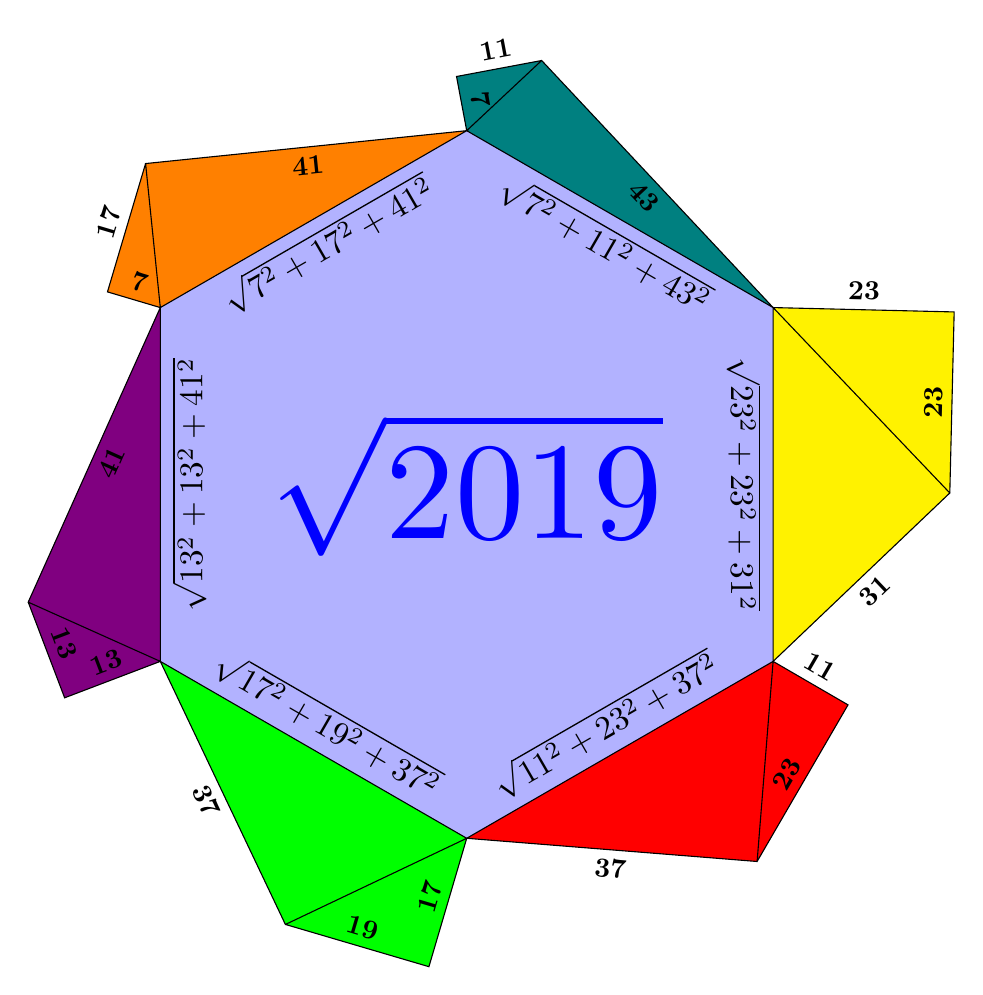
\begin{tikzpicture}[x=1mm,y=1mm]
		\pgfmathsetmacro{\r}{sqrt(2019)} % bán kính lục giác (mm)
		\fill[blue!30]
		(-30:\r)--(30:\r)--(90:\r)--(150:\r)--(210:\r)--(270:\r)--cycle;
		\node[scale=5,blue] (0,0) {$\sqrt{2019}$};
		\foreach \i/\a/\b/\c/\mau/\vitri in {
			0/23/23/31/yellow/below,
			1/7/11/43/teal/below,
			2/7/17/41/orange/below,
			3/13/13/41/violet/below,
			4/17/19/37/green/above,
			5/11/23/37/red/above}{
			\pgfmathsetmacro{\gone}{acos(\c/\r)}
			\pgfmathsetmacro{\gtwo}{atan(\b/\a)}
			\fill[\mau,draw=black] (60*\i+30:\r)--(60*\i-30:\r) node[black,sloped,midway,\vitri,scale=1.2]{$\sqrt{\a^2+\b^2+\c^2}$}--
			([turn]{180-\gone}:\c) node[black,midway,sloped,below]{\bfseries \c}--cycle--
			([turn]{180+\gtwo}:\a) node[black,midway,sloped,above]{\bfseries \a}--
			([turn]-90:\b) node[black,midway,sloped,above]{\bfseries \b};
		}
	\end{tikzpicture}
\end{document}